\section{Experiments}
\label{Sec:Experiments}

% This section evaluate Cerberus by answering several key questions.
% \begin{itemize}
%         \item \textbf{Q1}: will Cerberus improve application performance
%                 by utilizing burst buffer nodes?
%         \item \textbf{Q2}: Will job demand on burst buffer affect Cerberus?
%                 Why bother to divide the job execution into 3 phases?
%         \item \textbf{Q3}: Can dynamic programming based optimization
%                 help Cerberus further
% improve application performance?
% \end{itemize}
% Our newly developed event-driven simulator, BBSim, is used to simulating
% the Trinity system described later.

We evaluate Cerberus through a series of experiments with BBSim.
The experimental results give answers to three key questions.
\begin{itemize}
        \item \textbf{Q1}: Does the use of burst buffer 
        improve both system-level and job-level performance?
        \item \textbf{Q2}: What is the benefit of using 
        multiple queues to schedule jobs in a finer granularity than the single queuing system such as SLURM and PBS?
        \item \textbf{Q3}: What is the performance gain achieved 
        by the optimization proposed in section~\ref{SubSec:OptStageIn}-\ref{SubSec:OptStageOut}?
\end{itemize}

%traces
Our experiments are based on trace-driven simulation.
The Trinity system simulated by BBSim can be driven 
by workload trace collected from production systems.
%Since Trinity is not available to use at present, 
%there is no workload traces from Trinity available for our study.
In this paper, we use the workload trace collected from the Intrepid, a IBM Blue Gene/P system. 
The trace file contains 68,936 jobs
submitted to the system from January to September in 2009~\cite{Tang:IPDPS:2010}.
For each job, its log contains information such as submitted time, expected runtime, wait time, user ID, group ID, etc.
We patched three fields to each job's log entry: the amount of input data $data\_in$,
the total amount of written data for checkpointing $data\_run$
and the amount of output data $data\_out$.
We assume $data\_run$ and $data\_out$ follows the uniform distribution with a
lower bound of 1 TB and a upper bound of 60 TB;
$data\_in$ follows the uniform distribution between 1 GB and 30 GB~\cite{Liu:MSST:2012}.

% metric
We use three commonly used scheduling evaluation metrics,
\textit{job response time}, \textit{job waiting time} and \textit{system throughput}.
Job response time is the time duration between the job submission and its completion,
which is the major concern from user's perspective. 
Job waiting time is the aggregated wait time that a job stays in all three queues.
System throughput is defined as the number of jobs finished in
a fixed time period (500 seconds).


\subsection{Utilizing Burst Buffer Versus Direct I/O}
\label{Sec:Sim:DirectIOvsBB}

We examine the scheduling performance when 
jobs perform I/O operation in two different ways, 
namely, \textit{utilizing burst buffer} and \textit{Direct I/O}.
In the Trinity architecture, parallel file system (PFS) is mounted to all the compute nodes,
applications have the option to bypass the burst buffer 
and to use the file system directly for their I/O operations.
We refer this scenario as \textit{Direct I/O}. 
Apparently, the performance of \textit{Direct I/O}
is limited by the bandwidth of the I/O nodes. 

Figure~\ref{Fig:DirectIOvsBBResponse} compares CDFs of job response
time on the burst-buffer-enabled system and the traditional system (Direct I/O).
For the burst-buffer-enabled system, the job response time is bounded by 376,443.12 seconds.
However, the worst case of Direct I/O is catastrophic, 
i.e., a job takes 889,239.20 seconds to finish,
which is 2.36 times slower than the slowest non-responsive job
in the burst-buffer-enabled system.
In average, \textit{nearly 99\%} of the jobs scheduled on the burst-buffer-enabled system
respond faster than the traditional system without burst buffer, because the burst buffer can mitigate the I/O gap between I/O nodes and compute nodes.


Figure~\ref{Fig:DirectIOvsBBWait} reveals the aggregated job waiting time.
Note that in the case of Direct I/O, jobs only request compute nodes.
Thus, the waiting time is the duration between the job submission and the job starting time.
The difference of the worst case waiting time in the both systems is drastic.
On the system without burst buffer nodes, the waiting duration in the worst case is 3.02 times
slower than the worst case in the burst-buffer-enabled system.
The upper bound of the waiting duration for the burst buffer systems is about 285,254 seconds.
Because burst buffer has better ability to absorb checkpoint operations and data moving in/out,
the execution pipeline of job series is significantly fast.
Statistically, \textit{more than 80\% jobs have less waiting time if they utilize burst buffer.}

Figure~\ref{Fig:DirectIOvsBBThroughput} shows the system throughputs.
As indicated by the bar chart, \textit{the ratio of the average throughput between the two systems is 2.36}, i.e.,1.575 to 0.667.
It takes 889,239 seconds for the system without burst buffer nodes to
complete the workload. We pick a specific job with ID \#1150 from the workload, and observe its
waiting time in both cases.
Job \#1150 requested 256 compute nodes and 59 TB data space.
It started in the 1,126 second, but waited for 827,241 seconds.
In contrast, for the burst-buffer-enabled system, the same job accomplished the same workload in 376,443 seconds, and the waiting time and the response time of job \#1150
are significantly reduced, i.e., 272,741 and 376,026 seconds respectively.


\begin{figure*}[t]
        \centering
        \subfloat[Job Response Time] {
                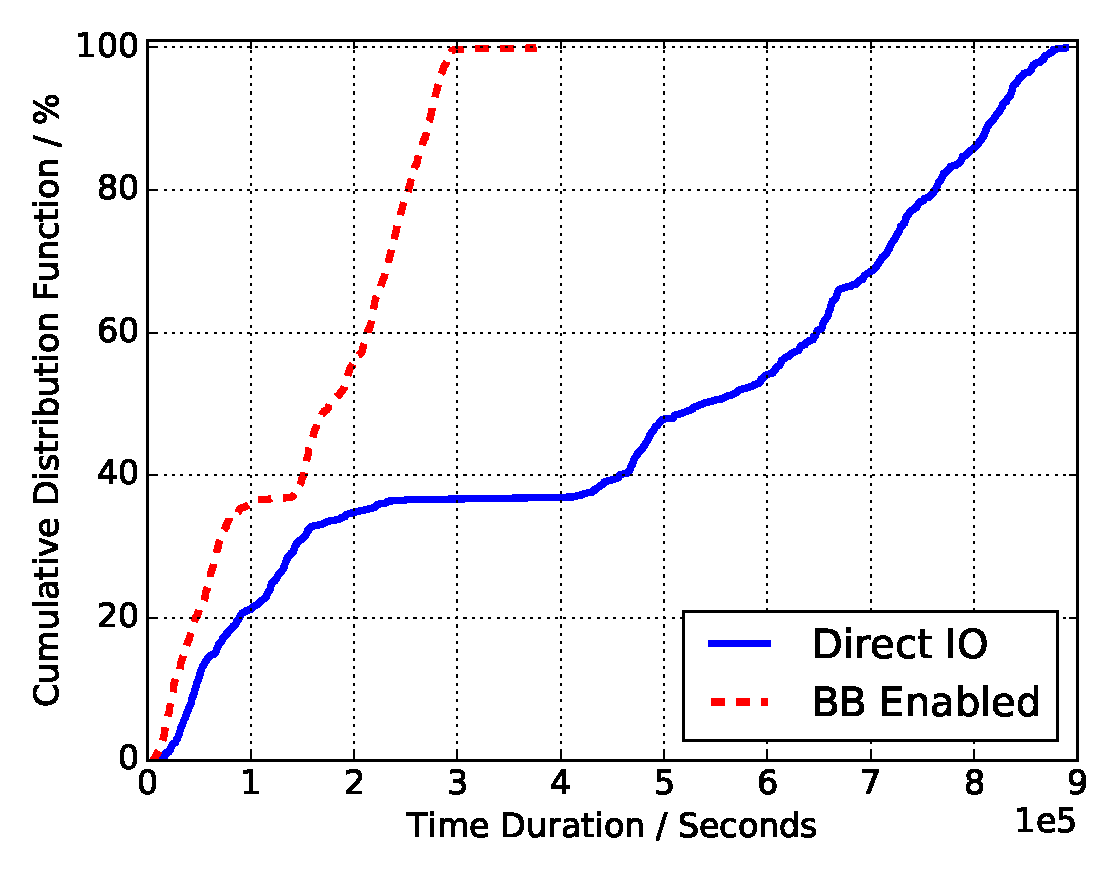
\includegraphics[width=2.2in]{IOvsBBFigures/1000jobs_direct_vs_bb_response}
                \label{Fig:DirectIOvsBBResponse}
        }
        \subfloat[Job Aggregated Wait Time] {
                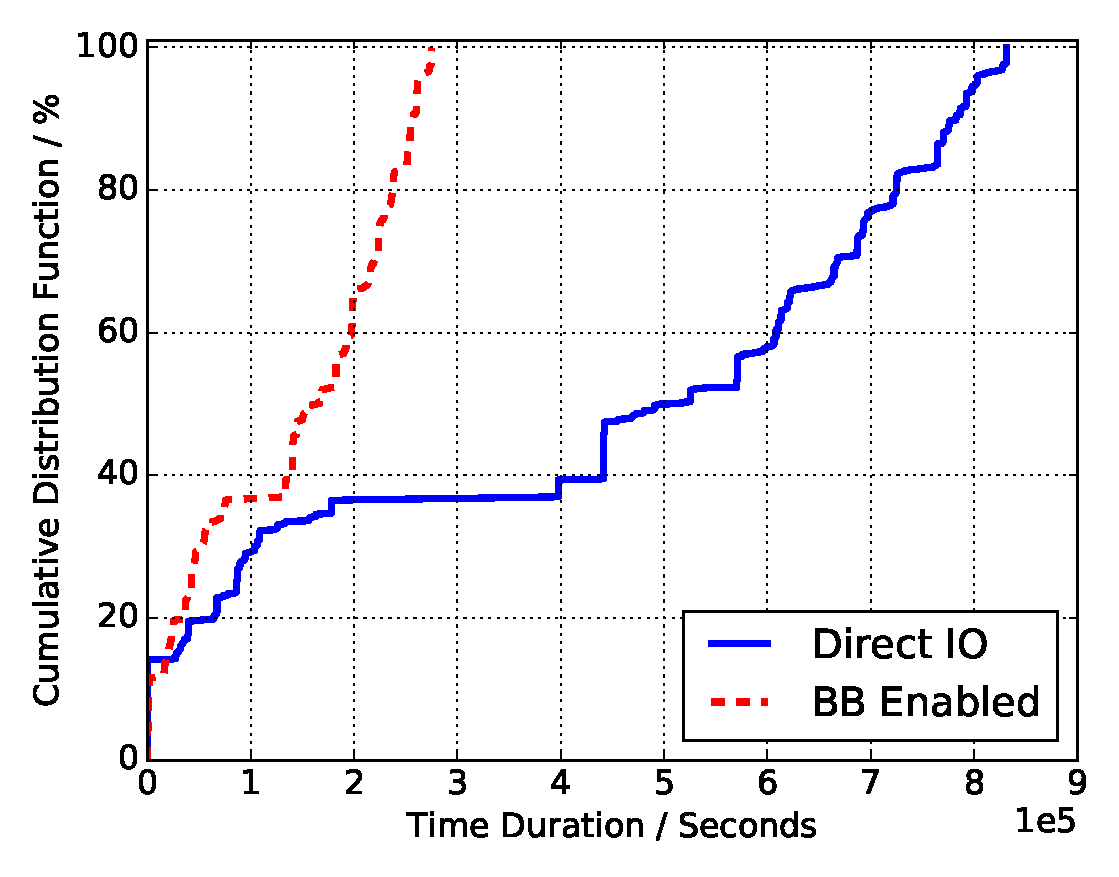
\includegraphics[width=2.2in]{IOvsBBFigures/1000jobs_direct_vs_bb_wait}
                \label{Fig:DirectIOvsBBWait}
        }
        \subfloat[System Throughput] {
                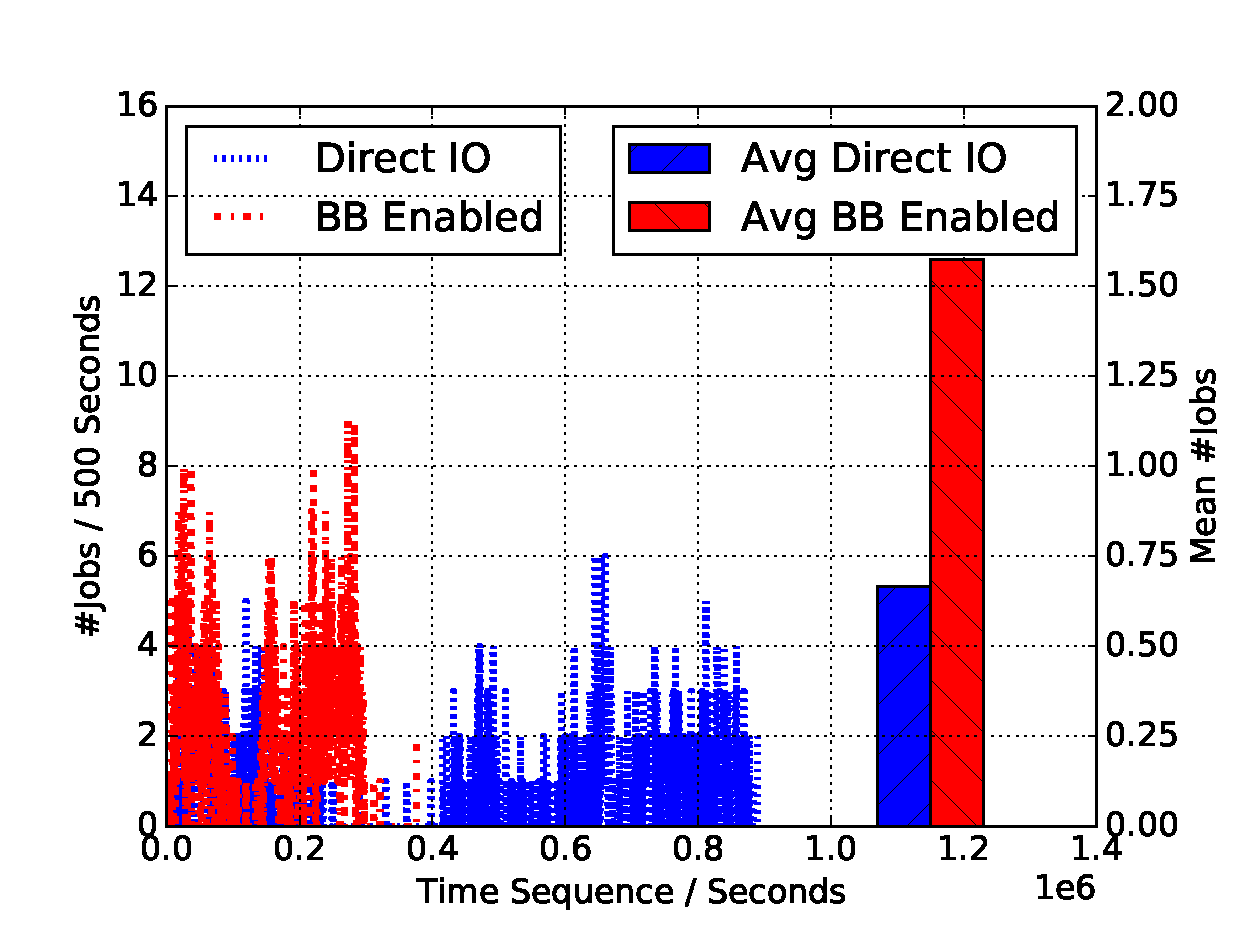
\includegraphics[width=2.5in]{IOvsBBFigures/1000jobs_direct_vs_bb_throughput}
                \label{Fig:DirectIOvsBBThroughput}
        }
        \caption{The comparison of scheduling performance between job utilizing burst buffer and conducting Direct I/O. In (c), on the left, the system throughput is presented in time sequence; the average system throughput is presented on the right. }
        \label{Fig:DirectIOPerformance}
\end{figure*}

%\begin{figure}[!t]
        %\centering
        %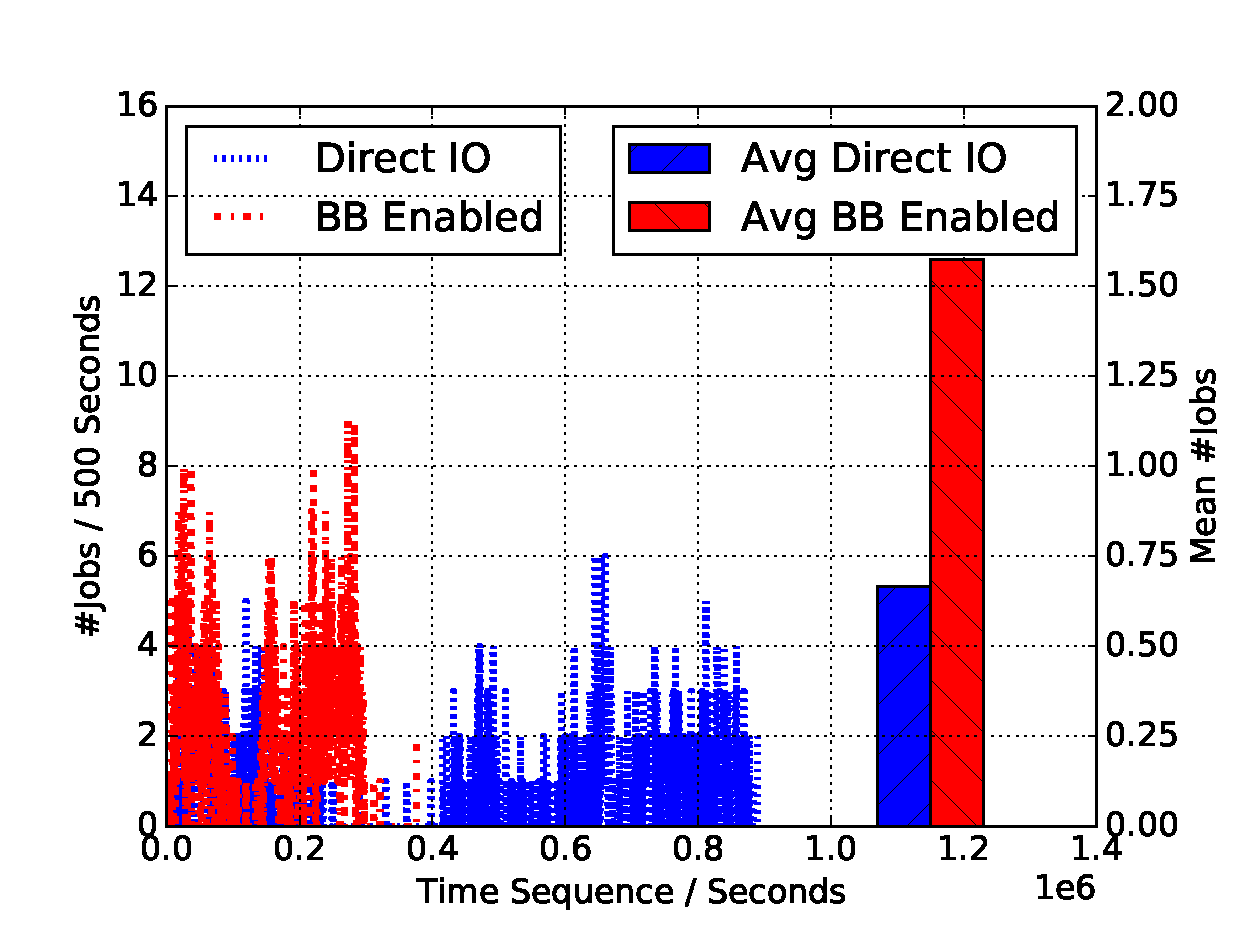
\includegraphics[width=3.2in]{IOvsBBFigures/1000jobs_direct_vs_bb_throughput}
        %\caption{System Throughput, IO Node Only vs. Burst Buffer System}
        %\label{Fig:DirectIOvsBBThroughput}
%\end{figure}
In short, the above experiments allow us to answer Q1.
That is, \textit{the use of burst buffer can improve both system-level and job-level performance.}
%Based on the above comparison, we can answer question \textbf{Q1}: 
%by utilizing burst buffer nodes,
%both the job-level and system-level performance can be significantly improved.
\textit{The execution of 99\% jobs will be expedited, 
80\% of jobs will suffer less wait time,
and the average system throughput will be improved as much as 136\%.}


\subsection{Cerberus Versus SLURM}
\label{Sec:Sim:CerberusVsSlurm}
We investigate the performance of scheduling jobs in different scheduling frameworks shown in Figure~\ref{Fig:CompareSlurmCerberus}.
As we discussed before, Cerberus is designed for scheduling the three-phase modeled jobs. 
It makes scheduling decisions in finer granularity than SLURM and PBS.
In Figure~\ref{Fig:3Pvs1PPerformance}, the scheduling results based on three job models
are presented:
\begin{itemize}
        \item \textbf{SLURM/PBS}: Jobs are submitted with the total burst buffer demand,
        and they are scheduled by a single queue.
	As a result, scheduler makes scheduling decision only once for each job.

        \item \textbf{Reduced Cerberus}: Jobs are also submitted with the total burst buffer demand,
        but their lifetime are divided into three phases and scheduled by three queues.
        In other words, this is the case that user provide less information to Cerberus.
        
        \item \textbf{Cerberus}: Jobs are submitted with the detailed burst buffer demand in each phase and are scheduled by Cerberus.

\end{itemize}
We assume the overall burst buffer demand in SLRUM/PBS and Reduced Cerberus is
$\max \{data\_in, data\_out, data\_run\}$.
The scheduling policy used in this experiment is just first-come first-serve.

When comparing the scheduling results of SLURM and Reduced Cerberus,
both of which only have the overall burst buffer demand of each job,
more than 60\% of the jobs in Reduced Cerberus finish faster than the jobs scheduled by
SLURM.
The slowest three-phase-modeled job takes 418,927 seconds to finish in Reduced Cerberus,
while the slowest job scheduled by SLURM takes about 492,591 seconds to finish.
The improvement is about 14.95\% in the worst case scenario.
The explanation is: In the single-queue SLURM, burst buffer nodes
are exclusively taken by the scheduled jobs throughout their entire lifetime.
In contrast, Cerberus reclaims the burst buffer multiple times;
It also releases the burst buffer nodes and the CPU resources at the earliest possible time, 
utilizing more system resources.
%Finally, when comparing the cases of 3-Phase-3D with 3-Phase-1D, we find another advantage of our 3-phase model.

In addition, if users can provide fine-grain information of data I/O demands,
Cerberus can coordinate three queues and make scheduling decision separately to achieve better scheduling results.
With burst buffer triple, Cerberus knows each job's demand during different phases.
The worst absolute response time is less than 379,026 seconds.
This is about 10.24\% improvement to Reduced Cerberus.
Even when Cerberus only knows the upper bound of data demand,
it is 23.66\% better than the slowest single-queue system.
In average, \textit{more than 80\% of the multiple-queued jobs
finish earlier than jobs in single-queue system.}
Meanwhile, \textit{more than 60\% of the jobs take less time if user
specifies burst buffer triple.}

We now investigate the detailed waiting time to understand why the scheduling results in Cerberus
are better than the naive integration of the batch scheduler with the burst buffer constraints.
Figure~\ref{Fig:3Pvs1PWaitRun} shows the waiting time, that is, how long a job spent in the running queue.
There are three queues in Cerberus.
Correspondingly jobs in Cerberus have three kinds of waiting time: waiting input, waiting running, and waiting output time.
%Figure~\ref{Fig:3Pvs1PWaitIn} shows the time job spend in inputing queue,
%Figure~\ref{Fig:3Pvs1PWaitOut} the time job spend in outputing queue.
For single-queue scheduler the waiting time in Figure~\ref{Fig:3Pvs1PWaitRun} is also the total waiting time.
We observe that (not shown in Figure~\ref{Fig:3Pvs1PPerformance}) the jobs did not
take much time either in the input queue $Q_I$ or in the output queue.
The upper bounds of time spent in the input queue, e.g. waiting time in $Q_I$, are 
2,500 seconds for both 3-Phase-1D and 3-Phase-3D modeled jobs.
This is because the input data are usually very small (e.g., tens of GB)
compared to the checkpointing data and the application output (e.g., tens of TB).
In contrast, in the worst case of SLURM, the job waiting time is 443,203 seconds,
because the scheduler makes a one-time decision based on the demand of the computer node and the maximum burst buffer.
%the upper bounds of time spent in output queue $Q_O$ are
%less than 5\% of the total waiting time of 1-phase-scheduler case
%for both 3-phases cases.
As for the time waiting for running, more than 60\% of the Cerberus-scheduled jobs are dispatched faster than SLURM.
The differences of the waiting time lead to the difference in response performance.

Figure~\ref{Fig:3Pvs1PThroughput} describes the system throughputs of the three different scheduler.
It helps us to examine the scheduling performance in time sequences.
For SLURM-scheduled jobs, we can see an obvious `throughput gap'
from 150,000 seconds to 200,000 seconds approximately.
The case of Reduced Cerberus is similar.
Cerberus runs counter to both previous cases.
Even though there is a throughput drop between 100,000 to 150,000 seconds,
it manages to make the system having a high throughput at the beginning and
later changes from 150,000 to 300,000 seconds.
In average, \textit{the throughput of Cerberus is 1.575 jobs / 500 seconds.}
It is 11.39\% higher than the reduced case (1.414 jobs / 500 seconds) and
23.68\% higher than SLURM/PBS(1.202 jobs / 500 seconds).
We believe that the results validate the indispensable three phase job model as well as
the multiple queue framework.
They also justifies the necessity of burst buffer triple.
We can now answer the question \textbf{Q2}:
\textit{the fine-grained multiple-queue scheduling benefits both job-level and system-level performance.}

\begin{figure*}[t]
        \centering
        \subfloat[Job Response Time] {
                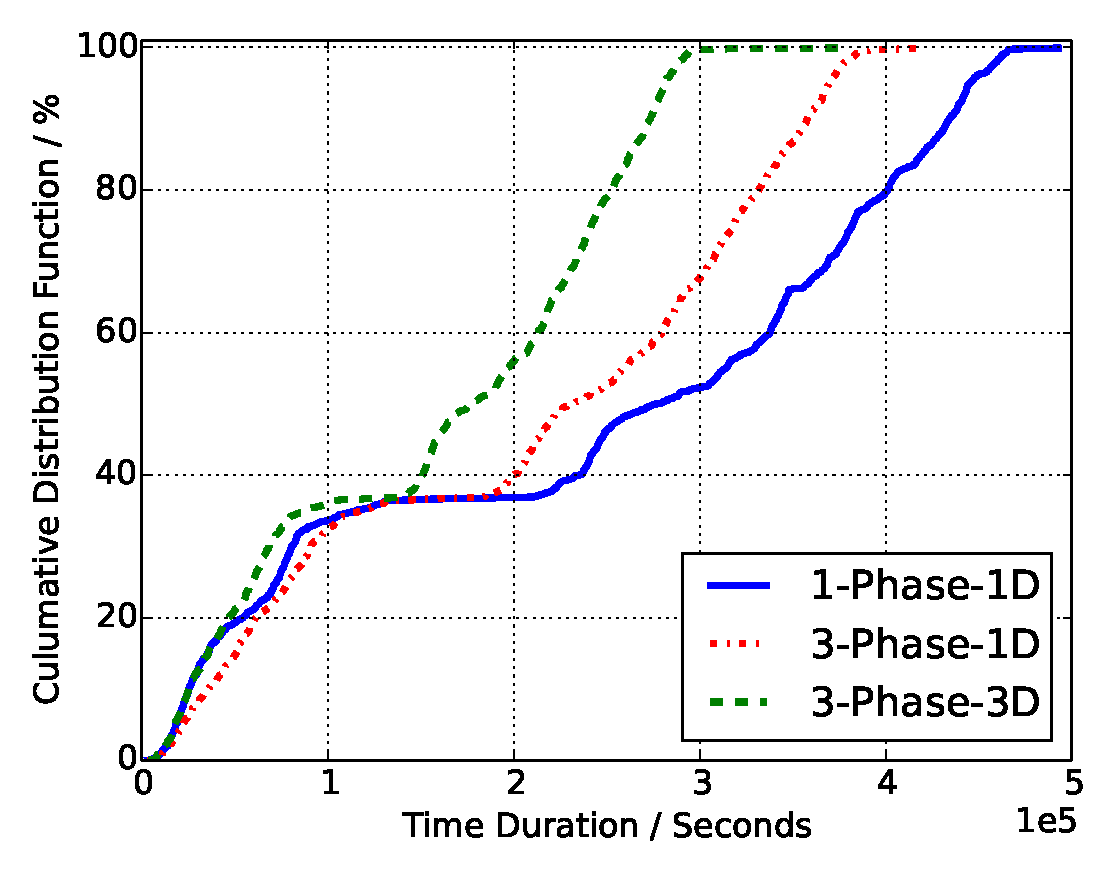
\includegraphics[width=2.2in]{3Pvs1PFigures/1000jobs_3p_vs_1p_response}
                \label{Fig:3Pvs1PResponse}
        }
        %\subfloat[Job Wait Time] {
                %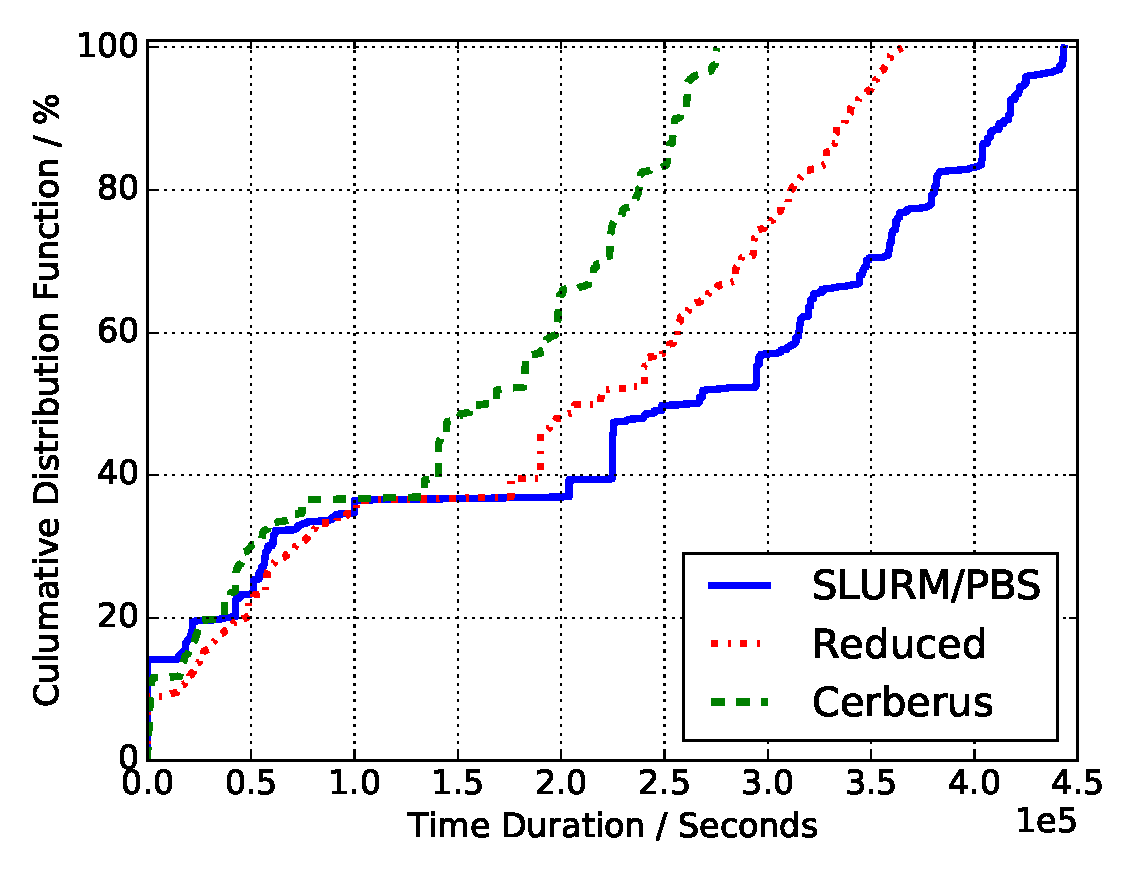
\includegraphics[width=3.2in]{3Pvs1PFigures/1000jobs_3p_vs_1p_wait}
                %\label{Fig:3Pvs1PWait}
        %}
        %\subfloat[Job Wait Input Time] {
                %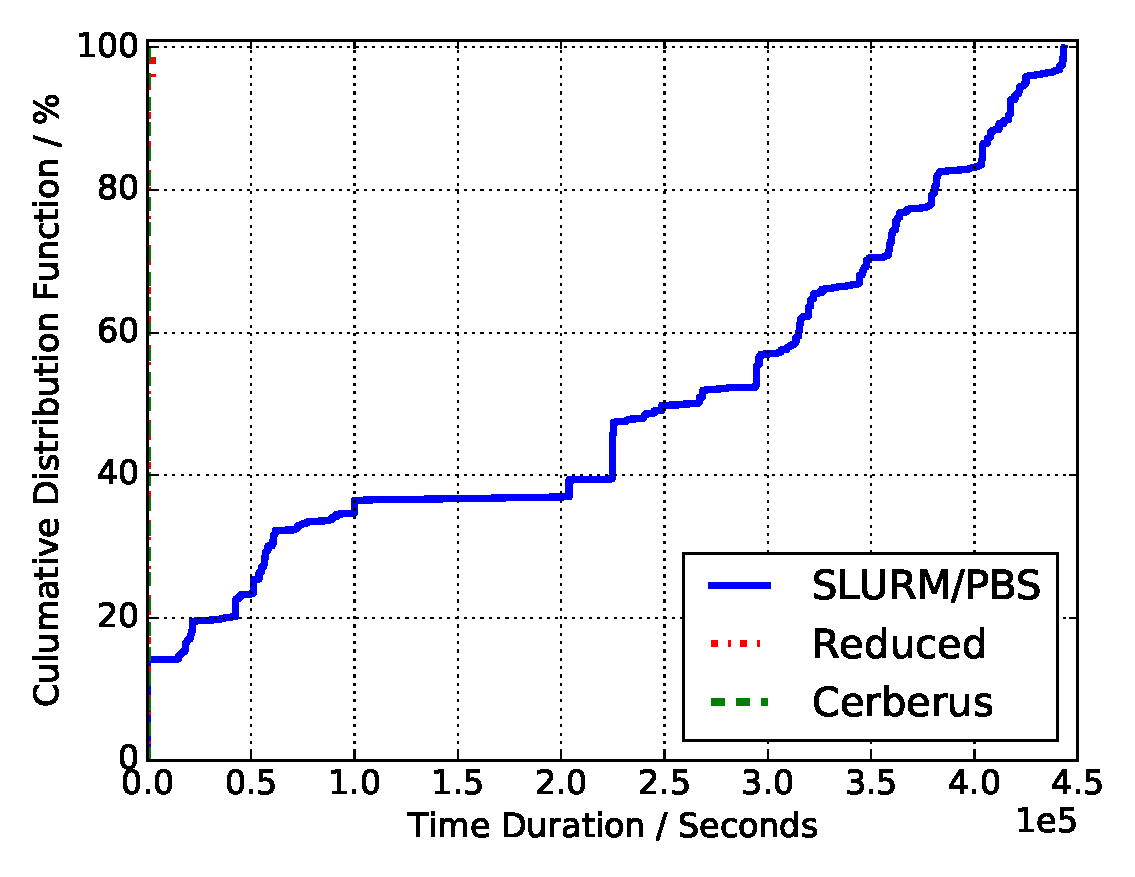
\includegraphics[width=2.3in]{3Pvs1PFigures/1000jobs_3p_vs_1p_wait_in}
                %\label{Fig:3Pvs1PWaitIn}
        %}
        %~
        \subfloat[Job Waiting Time in $Q_R$] {
                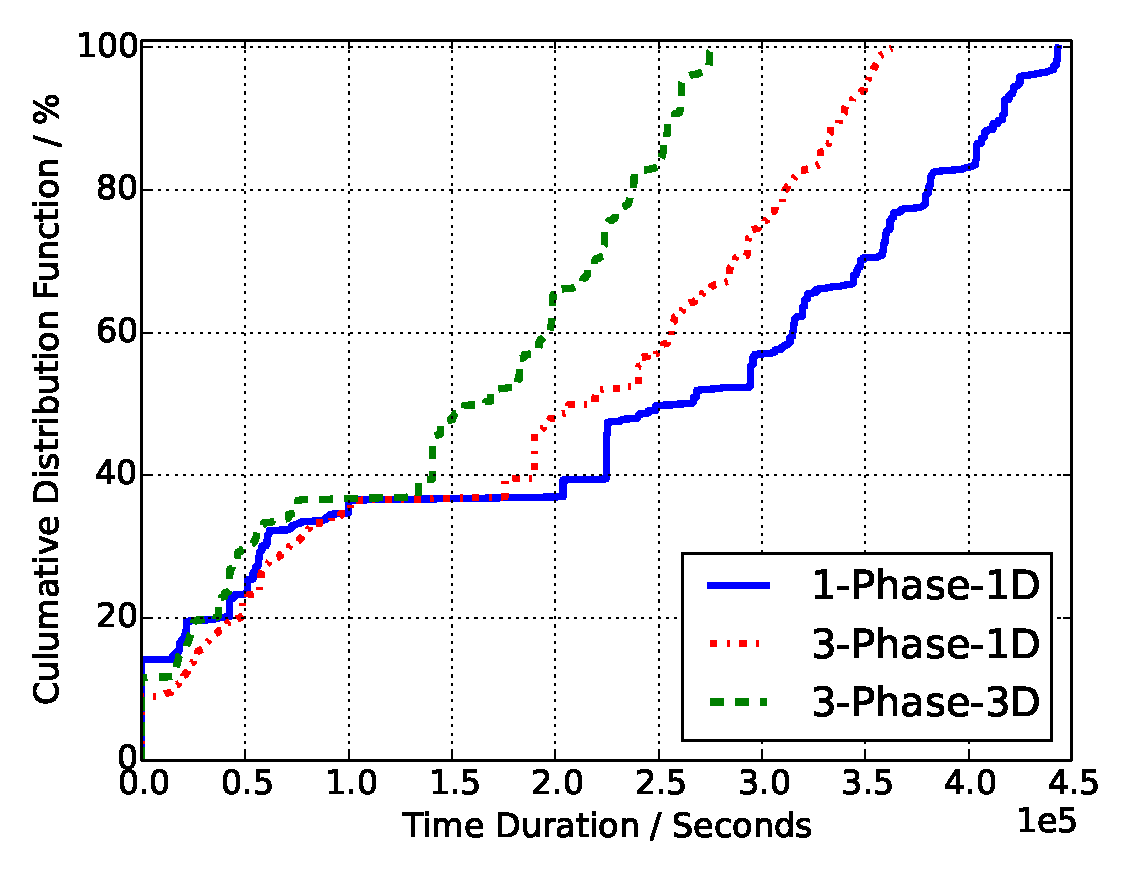
\includegraphics[width=2.2in]{3Pvs1PFigures/1000jobs_3p_vs_1p_wait_run}
                \label{Fig:3Pvs1PWaitRun}
        }
        \subfloat[System Throughput] {
                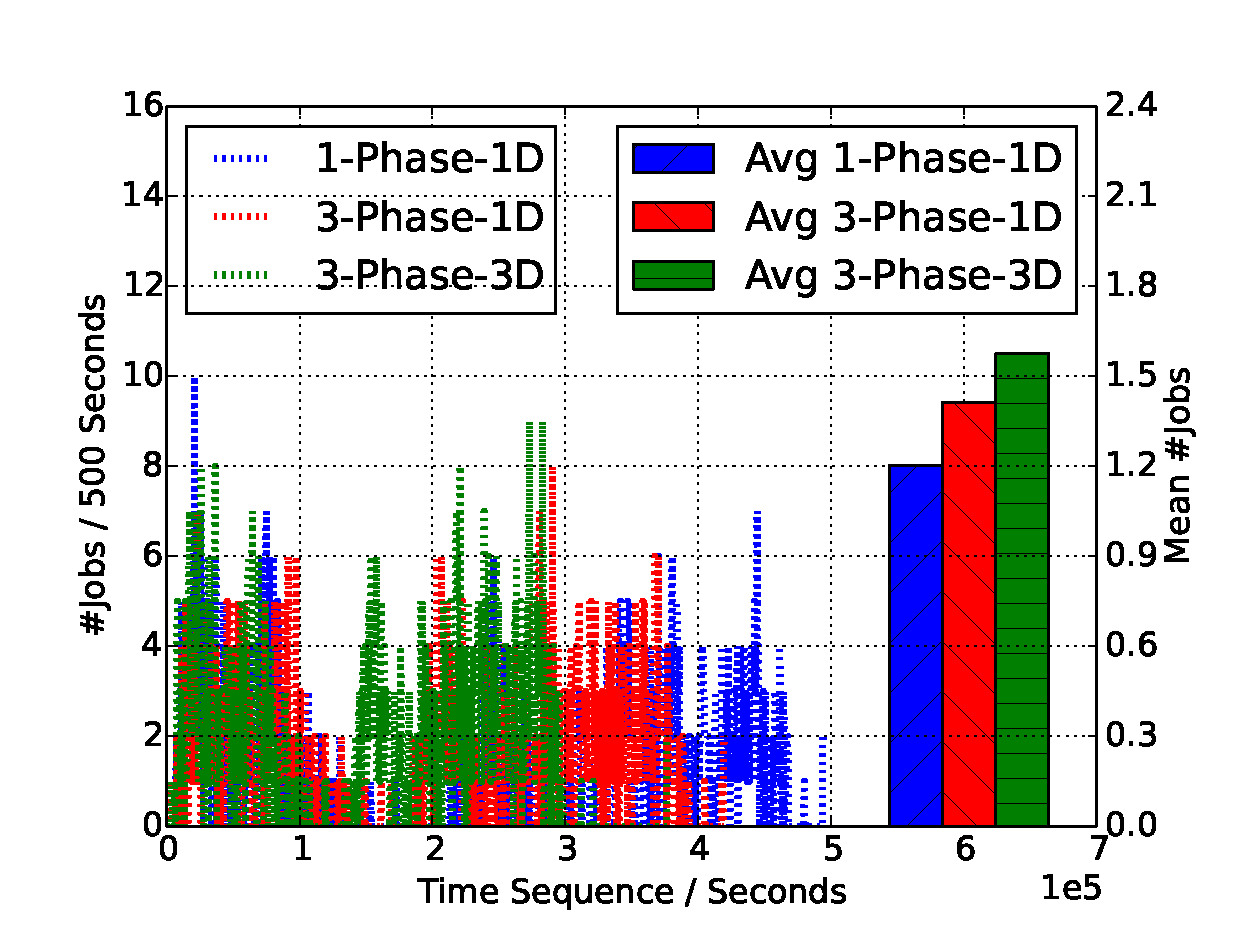
\includegraphics[width=2.5in]{3Pvs1PFigures/1000jobs_3p_vs_1p_throughput}
                \label{Fig:3Pvs1PThroughput}
        }
        \caption{The comparison of scheduling performance between using 3-phase model and 1-phase model. In (c), on the left, the system throughput is presented in time sequence; the average system throughput is presented on the right.}
        \label{Fig:3Pvs1PPerformance}
\end{figure*}

%\begin{figure}[!t]
        %\centering
        %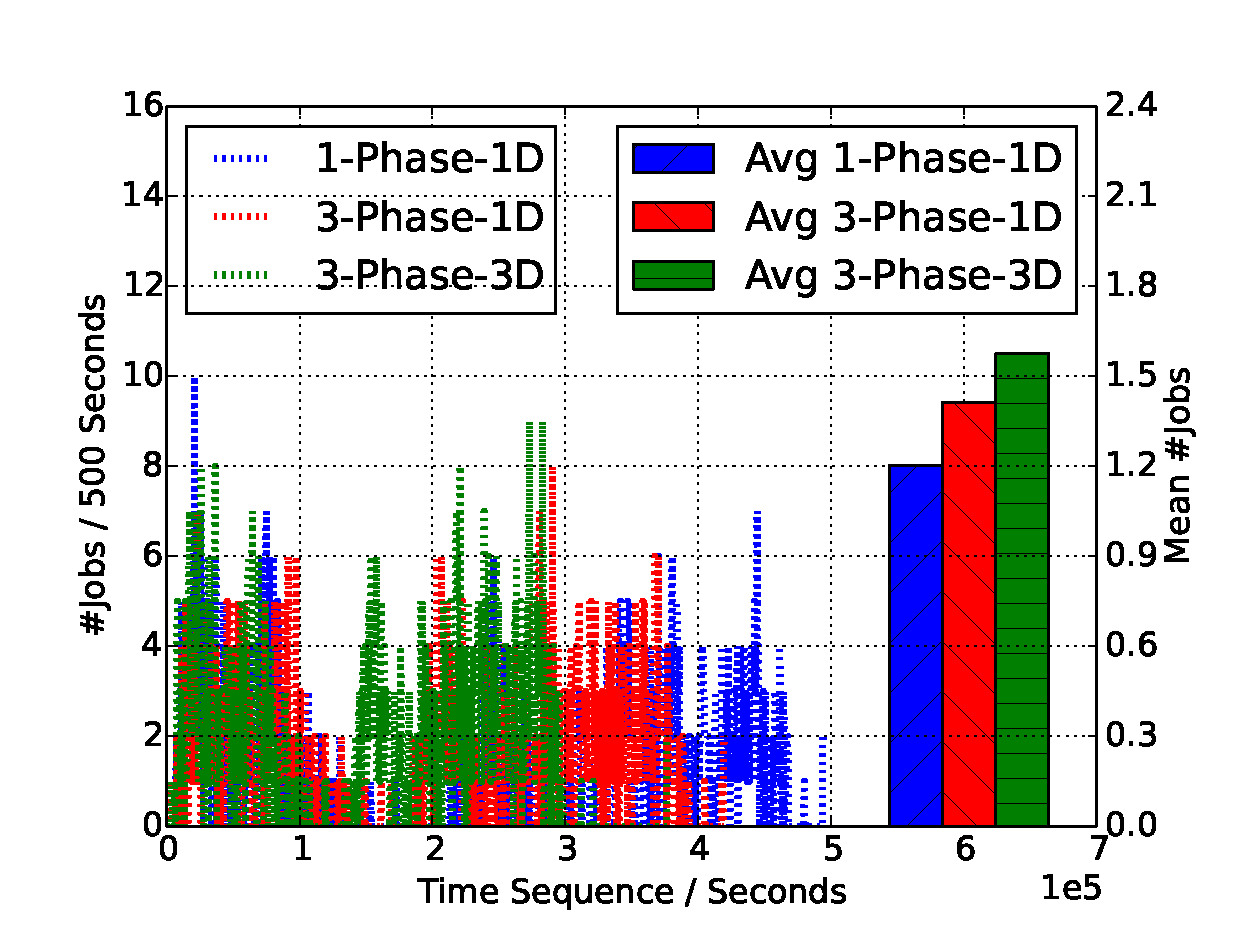
\includegraphics[width=3.2in]{3Pvs1PFigures/1000jobs_3p_vs_1p_throughput}
        %\caption{System Throughput, 1 Phase Model vs. 3 Phase Model}
        %\label{Fig:3Pvs1PThroughput}
%\end{figure}

\begin{figure*}[t]
        \centering
        \subfloat[Job Response Time] {
                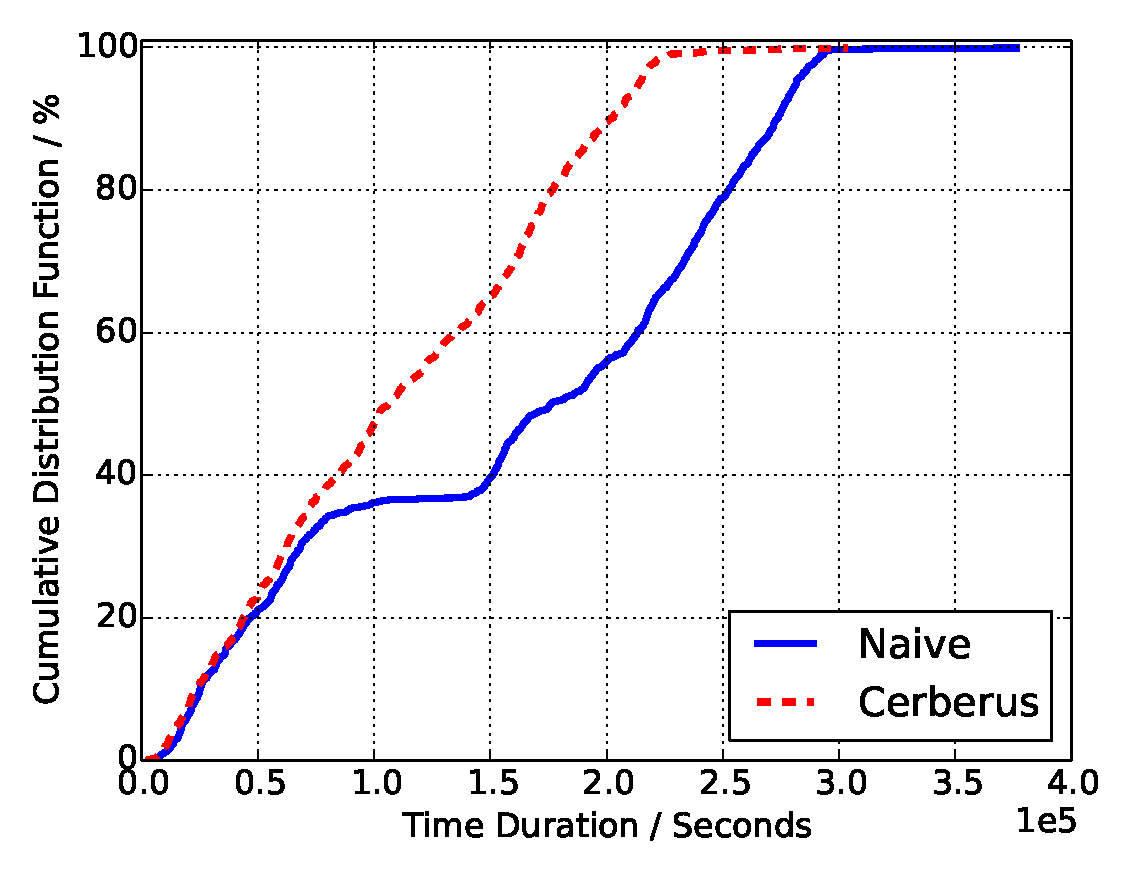
\includegraphics[width=2.2in]{DPvsFIFOFigures/1000jobs_dp_vs_fifo_response}
                \label{Fig:DPvsFIFOResponse}
        }
        \subfloat[Job Aggregated Waiting Time in $Q_R$] {
                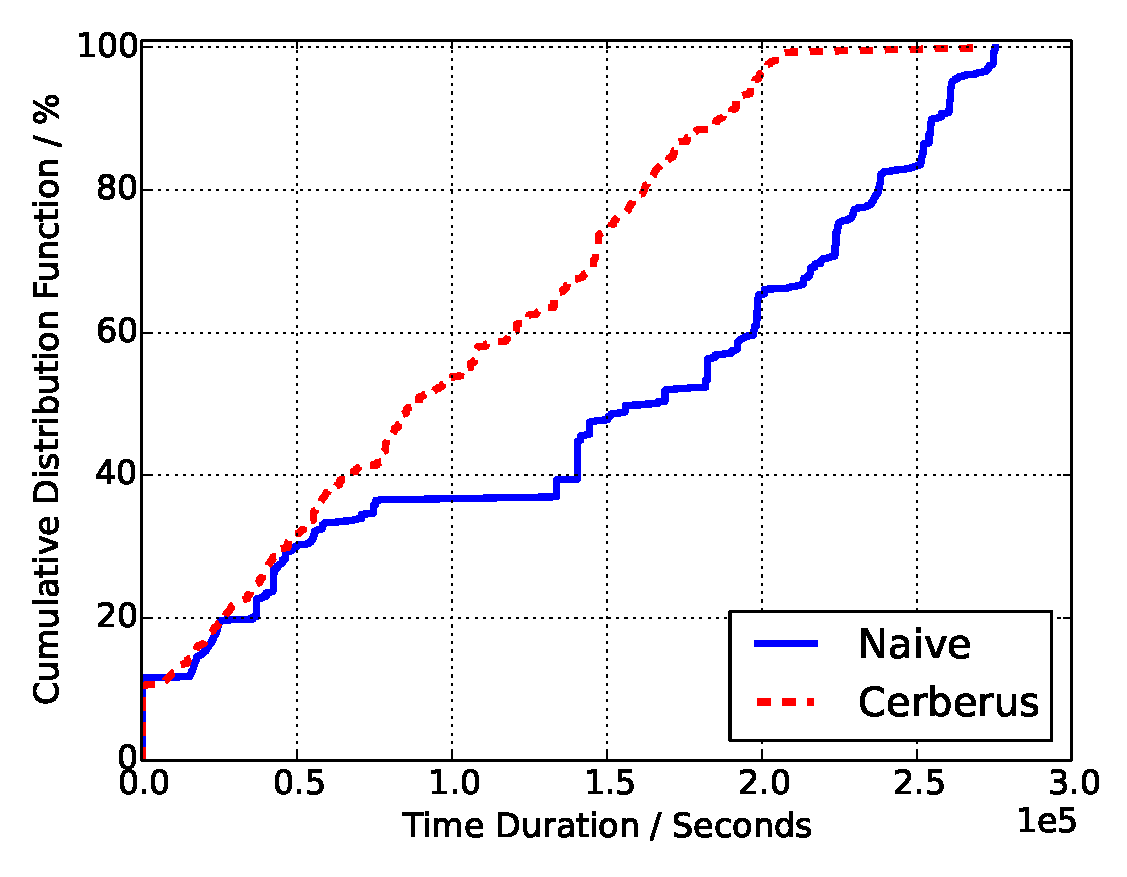
\includegraphics[width=2.2in]{DPvsFIFOFigures/1000jobs_dp_vs_fifo_wait_run}
                \label{Fig:DPvsFIFOWaitRun}
        }
        \subfloat[System Throughput] {
                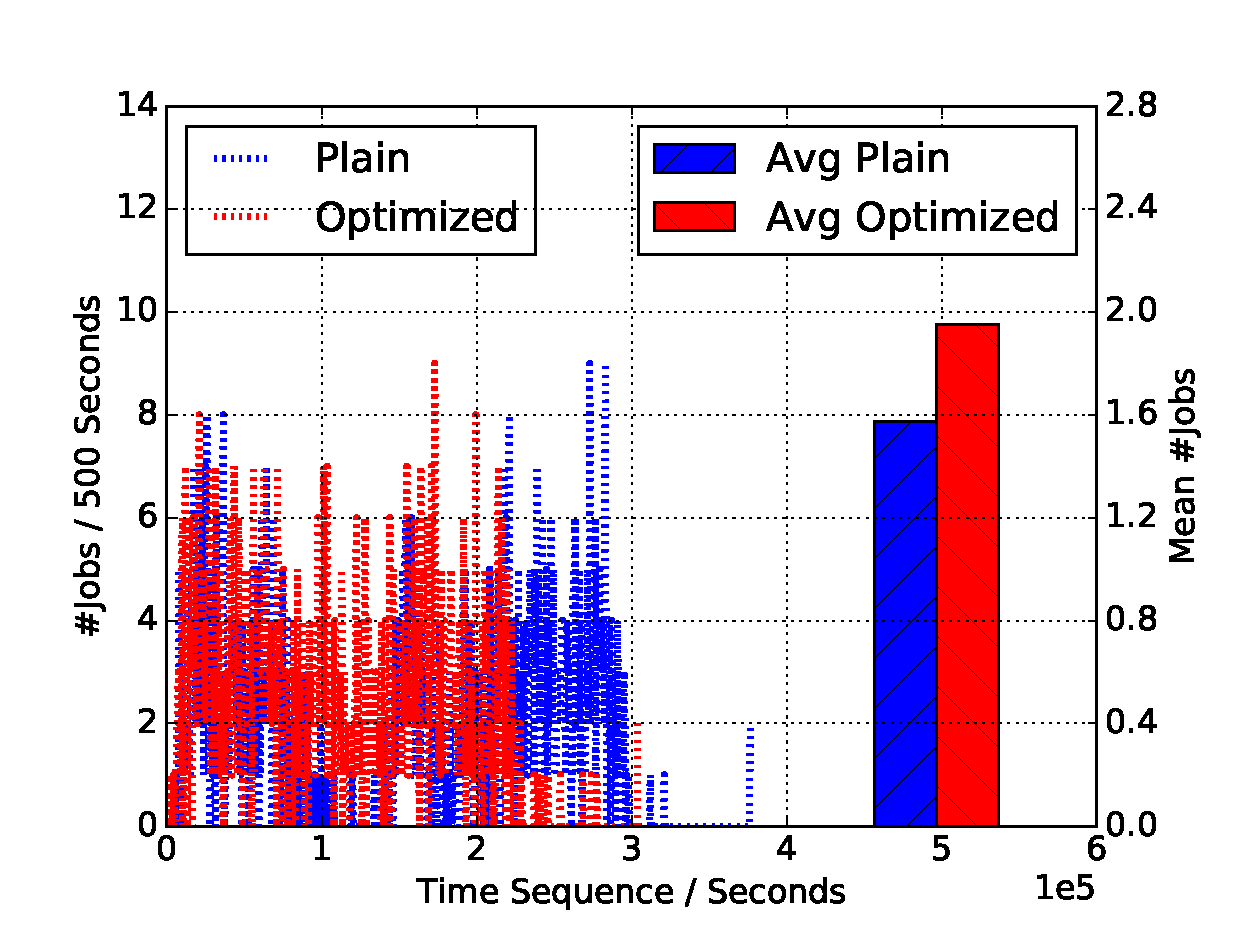
\includegraphics[width=2.5in]{DPvsFIFOFigures/1000jobs_dp_vs_fifo_throughput}
                \label{Fig:DPvsFIFOThroughput}
        }
        \caption{The comparison of scheduling performance obtained by Cerberus and a naive first-come, first-serve scheduling. In (c), on the left, the system throughput is presented in time sequence; the average system throughput is presented on the right.}
        \label{Fig:DPvsFIFOPerformance}
\end{figure*}

%\begin{figure}[!t]
        %\centering
        %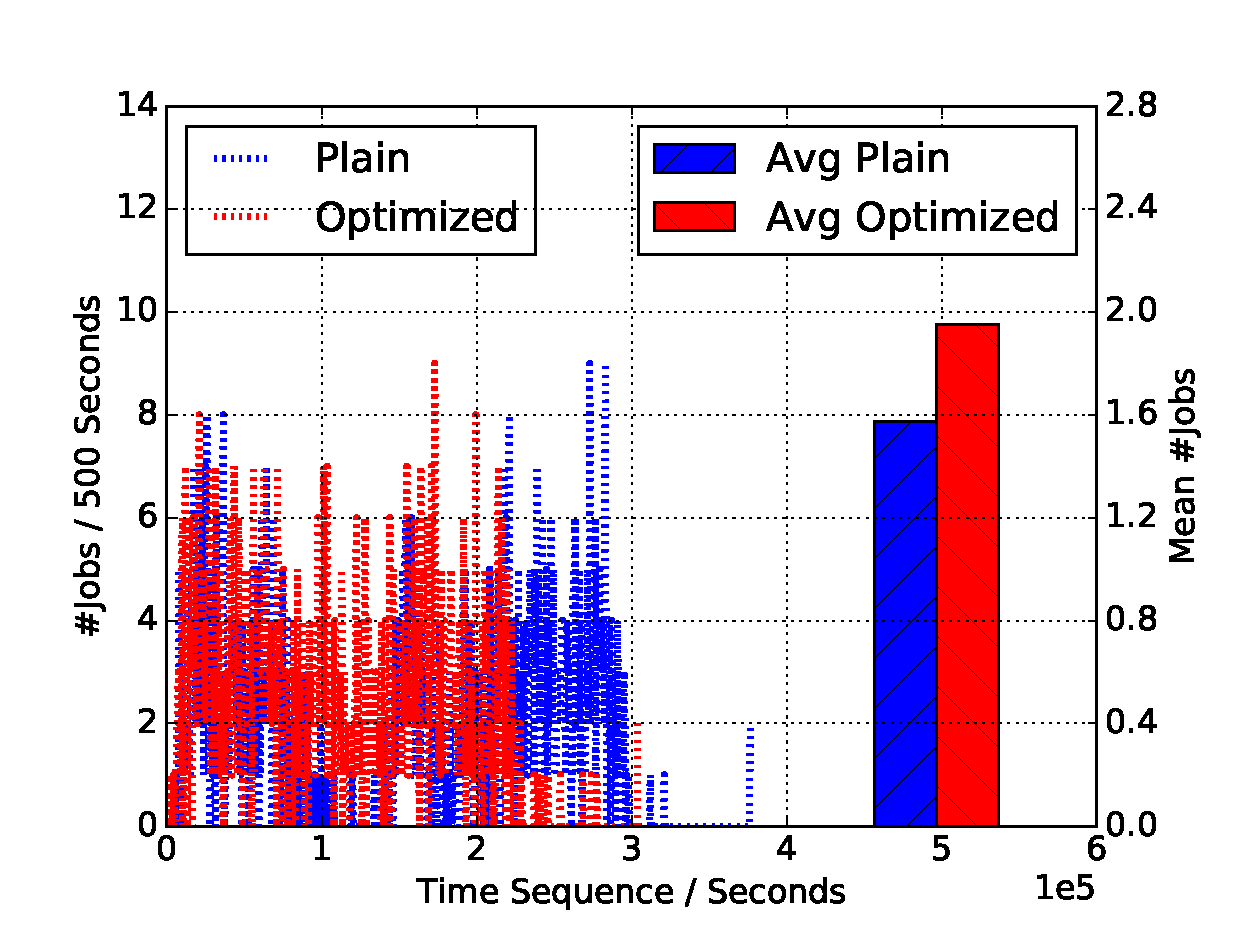
\includegraphics[width=3.2in]{DPvsFIFOFigures/1000jobs_dp_vs_fifo_throughput}
        %\caption{System Throughput, Optimized Cerberus vs. FCFS Cerberus}
        %\label{Fig:DPvsFIFOThroughput}
%\end{figure}


\subsection{Optimization Enhancement in Cerberus}

Cerberus adopts various algorithms when scheduling jobs in each queue. 
The optimization algorithms presented in section \ref{SubSec:OptStageIn} and \ref{SubSec:OptRunning} are integrated in Cerberus. 
In this section, we answer the question \textbf{Q3} by showing that
adopting optimization in each scheduling phase can bring further improvement
compared with a naive first-come first-serve strategy.
Specifically, in the stage-in and stage-out phases, Cerberus schedules the jobs in $Q_I$ and $Q_O$
according to the solution given by \equref{Equ:MaxTransferDataRecursion}.
For jobs in $Q_R$, Cerberus makes the scheduling decisions
based on the solution given by \equref{Equ:MaxProductRecursion}. %Algorithm~\ref{Alg:MaxCPU}.
We denote Cerberus with and without optimization
as \textbf{Optimized} and \textbf{Plain} respectively.

As indicated by Figure~\ref{Fig:DPvsFIFOResponse}, the job response time scheduled by Cerberus is reduced.
The most non-responsive job for Cerberus is job \#445, which takes 303,523 seconds to complete.
In contrast, job \#445 takes 376,026 seconds to finish in Plain Cerberus.
This is 19.28\% slower than the Optimized Cerberus.
When we consider the overall response time of the entire job set,
we observe that more than \textit{80\% of the jobs respond faster when Cerberus adopts optimizations}.

The time duration that an application is waiting for running
is plotted in Figure~\ref{Fig:DPvsFIFOWaitRun}.
The tail of Optimized Cerberus shows that a couple of jobs
spend very long time in the running queue.
This is because: First the jobs are submitted at the early middle phase
(job \#435 waits for 268,322 seconds).
Second, these jobs request a huge
amount of compute nodes (10240), but comparably less amount of burst buffer (7 TB for job \#435).
Third, there are jobs requesting a large number of cores but requesting
less running time and a larger amount of burst buffer.
For example, job \#434 requests 10,240 compute nodes but the expected running time
is only 3,600 seconds and it also requests 59 TB burst buffer.

As a result, Optimized Cerberus favors the jobs with less requesting time and larger burst buffer demand,
according to \equref{Equ:MaxProductRecursion}.
This is interesting because it is a potential flaw in the optimization-based policy:
Given that the users know the optimization objective of the scheduler,
it is possible for a user to cheat the scheduler with false demands.
%In other words, our optimization scheme, even though providing performance enhancement
%for the waiting time of 70\% jobs, is not strategy-proofness\cite{Ghodsi:NSDI:2011}


We can see the system throughputs under different scheduling objectives in Figure~\ref{Fig:DPvsFIFOThroughput} .
By adding optimization in Cerberus, it takes 303,940 seconds to finish the workload,
while Plain Cerberus takes 376,443 seconds to complete the same workload.
The worst case completion time improvement of Optimized version over Plain version is 19.26\%.
When we look at the time sequence of throughput,
we found that the peak value 9 jobs / 500 seconds can be finished when scheduled by Optimized Cerberus.
The peak throughput of the Plain Cerberus is also 9 jobs / 500 seconds.

The results in Figure~\ref{Fig:DPvsFIFOPerformance} answer question \textbf{Q3}: 
when Cerberus adopts optimization algorithms to schedule jobs,
the execution of 80\% jobs can be expedited; their wait time is also greatly reduced.
In the meanwhile, as plotted in Figure~\ref{Fig:DPvsFIFOThroughput},
\textit{Cerberus boots system throughput by as much as 23.87\%} (1.951 jobs / 500 seconds) in average.

It is important to point out that
though solving the optimization problem is theoretically NP-hard,
memorization technique enables Cerberus to perform online job scheduling.
In our simulation, it takes about 0.04 second in average for Cerberus to make a scheduling decision.


%Table~\ref{Tab:OptimizationTime} demonstrate that 
% % Memoization technique helps optimized Cerberus be able to schedule jobs online,
% % though solving the optimization problem is theoretically NP-hard.
% % For Optimized Cerberus, it solved about 8400 Problem~\ref{Equ:MaxTransferData} and
% % Problem~\ref{Equ:MaxProduct} when scheduling all the jobs in workload,
% % taking less than 370 seconds.
% % The time overhead of solving each optimization is about 0.04 seconds per time.

%\begin{table}[!t] 
        %\renewcommand{\arraystretch}{1.3}
        %\caption{Time Consumption in Dynamic Programming}
        %\label{Tab:OptimizationTime}
        %\centering
        %\begin{tabular}{l|c}
                %\hline
                %Optimization Policy Used & Optimized Cerberus\\
                %\hline
                %\hline
                %Simulation Run Time / seconds & 375.55\\
                %Optimization Run Time / seconds & 364.62\\
                %Total Number of Optimizations & 8406\\
                %\hline
        %\end{tabular}
%\end{table}


